\newpage
\thispagestyle{empty}

\textbf{\large Zadanie práce}

\textbf{Názov zadania}: Inteligentný asistent trénovania prezentačných schopností

\textbf{Názov v angličtine}: Intelligent assistant for training presentation skills

Ústav informatiky, informačných systémov a softvérového inžinierstva, FIIT STU

\textbf{Text zadania}: Z prezentovania pred publikom alebo na verejnosti mávajú hlavne menej skúsení rečníci rôzne obavy, napríklad či bude ich prezentácia dostatočne zaujímavá, zrozumiteľná, plynulá a bez chýb. Tieto obavy sú prirodzené, hlavne pokiaľ nemáme dostatok skúseností, či nie sme zvyknutí verejne vystupovať. Tieto obavy je možné zvládnuť vhodným tréningom.
Oboznámte sa s problematikou úspešného a efektívneho prezentovania a preskúmajte moderné prístupy trénovania prezentačných schopností. Analyzujte najčastejšie problémy, s ktorými sa stretávajú rečníci počas prezentovania, ako sú napríklad nesprávne využívanie neverbálnych a verbálnych prejavov. Identifikujte, ktoré nevhodné javy najviac ovplyvňujú kvalitu prezentácie a zapracujte ich do finálneho riešenia.
Navrhnite inteligentného asistenta na trénovanie prezentačných schopností, ktorý bude použitý pri nácviku verejných prezentácií a bude poskytovať spätnú väzbu na neverbálne a verbálne prejavy rečníka. Využite metódy spracovania obrazu a zvuku na detekciu nevhodných javov počas prezentácie. Na základe zistených javov navrhnite a implementujte systém odporúčaní, ktorý rečníkovi poskytuje spätnú väzbu a usmernenia na zlepšenie jeho prezentačných schopností. Navrhnuté riešenie implementujte a overte.
% 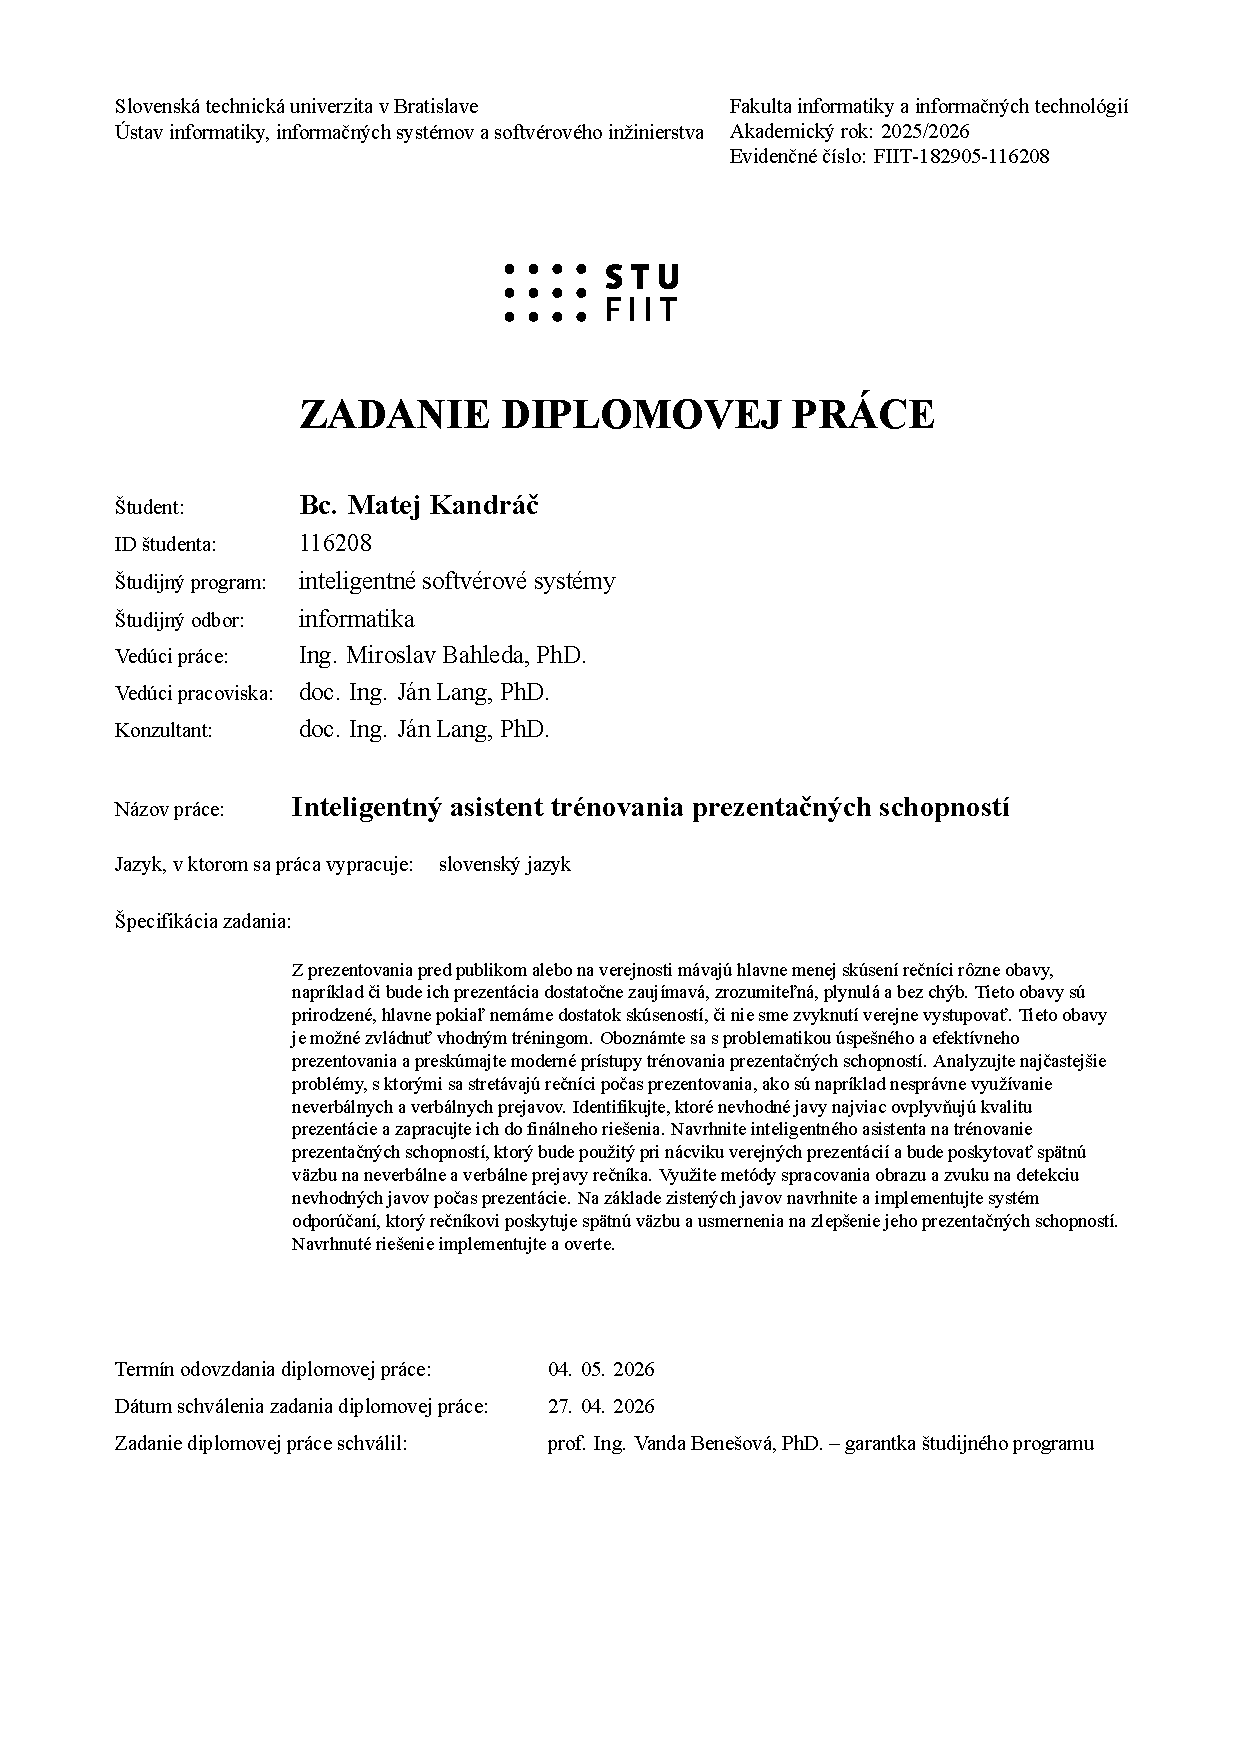
\includepdf[pages=1,scale=0.8]{assets/zadanie.pdf}
\newpage

\thispagestyle{empty}
\mbox{}
\newpage
\thispagestyle{empty}